\documentclass[11pt,class=report,crop=false]{standalone}
\usepackage[screen]{../python}


\begin{document}


%====================================================================
\chapitre{Programmation objet}
%====================================================================

\index{objet}
\index{programmation objet}

\objectifs{Avec \Python{} tout est objet : un entier, une chaîne, une liste, une fonction\ldots{} Nous allons voir comment définir nos propres objets.}


%%%%%%%%%%%%%%%%%%%%%%%%%%%%%%%%%%%%%%%%%%%%%%%%%%%%%%%%%%%%%%%%
%%%%%%%%%%%%%%%%%%%%%%%%%%%%%%%%%%%%%%%%%%%%%%%%%%%%%%%%%%%%%%%%

\begin{cours}[Programmation objet : la classe !]

\index{class@\ci{class}}
\index{programmation objet!classe}
\index{vecteur}

Un \defi{objet} est une entité qui regroupe à la fois des variables et des fonctions.
Le premier intérêt est qu'un objet est indépendant et auto-suffisant 
puisqu'il contient tout ce qu'il faut pour être utilisé, il permet d'éviter le recours aux variables globales par exemple. 


Un objet est défini comme une \defi{instance} d'une \defi{classe}, c'est-à-dire un élément d'une catégorie.
Voici un exemple de la vie courante : on considère la classe \emph{Chien}, alors mon chien \emph{Médor} est un objet, appartenant à la classe \emph{Chien}. Note que \emph{Chien} est un concept, mais que \emph{Médor} est bien réel.
Mon autre chien \emph{Foulcan} est aussi une instance de \emph{Chien}.

\medskip

Voici comment définir le début d'une classe \ci{Vecteur()} afin de modéliser des vecteurs de l'espace :
\begin{lstlisting}
class Vecteur:
    def __init__(self,x,y,z):
        self.x = x
        self.y = y
        self.z = z     
\end{lstlisting} 
Pour l'instant un vecteur est un concept auquel sont rattachés trois nombres $(x,y,z)$. Le mot \ci{self} fait référence à l'objet lui-même mais dont on ne connaît pas encore le nom (ce sera \ci{V} ou bien \ci{V1}, \ci{V2}\ldots).



Et voici un objet défini à partir de cette classe :
\mycenterline{\ci{V = Vecteur(1,2,3)}}
Cet objet possède trois \defi{attributs} :
\mycenterline{\ci{V.x} \qquad \ci{V.y} \qquad \ci{V.z}}
qui valent ici respectivement $1$, $2$ et $3$. Autre exemple, le calcul \ci{V.x + V.y + V.z} renvoie $6$.
Je peux changer une de ces valeurs comme pour une variable classique (même si ce n'est pas la manière recommandée), par exemple :
\mycenterline{\ci{V.x = 7}}
Maintenant  \ci{V.x + V.y + V.z} vaut $12$.



Tu peux définir plusieurs objets qui seront indépendants les uns des autres :
\mycenterline{\ci{V1 = Vecteur(1,2,3)} \qquad \ci{V2 = Vecteur(1,0,0)}}
Ainsi par exemple \ci{V1.y} vaut $2$, \ci{V2.y} vaut $0$.

\end{cours}
 

\begin{cours}[Programmation objet : de la méthode.]

\index{methode@méthode}
\index{programmation objet!methode@méthode}


On a vu comment attribuer des variables à un objet. Nous allons voir comment lui associer des fonctions.
Pour un objet, une fonction associée s'appelle une \defi{méthode}.

Si on reprend l'exemple de la classe \emph{Chien}, on pourrait lui associer une méthode \emph{Viens\_ici\_!}.
On peut donc demander \emph{Médor.Viens\_ici\_!} ou bien \emph{Foulcan.Viens\_ici\_!} pour appeler chacun de nos chiens.

\medskip

Complétons notre classe \ci{Vecteur()} pour lui associer trois nouvelles méthodes :
\begin{lstlisting}
class Vecteur:
    def __init__(self,x,y,z):
        self.x = x
        self.y = y
        self.z = z

    def norme(self):
        N = sqrt(self.x**2 + self.y**2 + self.z**2)
        return N

    def produit_par_scalaire(self,k):
        W = Vecteur(k*self.x,k*self.y,k*self.z)
        return W

    def addition(self,other):
        W = Vecteur(self.x+other.x,self.y+other.y,self.z+other.z)
        return W
\end{lstlisting} 

\begin{itemize}
  \item La méthode \ci{norme()} renvoie la norme $\sqrt{x^2+y^2+z^2}$ d'un vecteur $(x,y,z)$ (il faut importer le module \ci{math}). 
  Par exemple pour \ci{V = Vecteur(1,2,3)}, on demande sa norme par la commande :
  \mycenterline{\ci{V.norme()}}
qui renvoie ici une valeur approchée de $\sqrt{14} = 3.74\ldots$  

   La méthode \ci{norme()} est définie comme une fonction classique, le paramètre prend le nom de \ci{self}
   et correspond à l'objet (le vecteur \ci{V} pour notre exemple). On récupère les coordonnées par
   \ci{self.x}, \ci{self.y}, \ci{self.z} (pour notre exemple cela correspond à \ci{V.x}, \ci{V.y}, \ci{V.z}).
  
  
  \item La méthode \ci{produit_par_scalaire(self,k)} multiplie les coordonnées d'un vecteur par un réel $k$.
  Par exemple pour \ci{V = Vecteur(1,2,3)} alors la commande :
  \mycenterline{\ci{W = V.produit_par_scalaire(7)}}
définit un nouvel objet \ci{Vecteur()}, noté \ci{W}, représentant le vecteur $\vec w = (7,14,21)$.
Maintenant \ci{W} est un objet de classe \ci{Vecteur()} comme les autres et on peut par exemple calculer sa norme par \ci{W.norme()}. 
La méthode \ci{produit_par_scalaire()} est définie à l'aide de deux paramètres. Le premier est obligatoirement \ci{self} et fait toujours référence à l'objet traité. Le second est ici le facteur $k$. Lorsque l'on appelle la méthode cela devrait être \ci{produit_par_scalaire(V,7)} mais la syntaxe des objets est \ci{V.produit_par_scalaire(7)}
(le premier argument passe devant le nom de la méthode, les autres arguments sont décalés).


  \item La méthode \ci{addition(self,other)} renvoie le vecteur somme de deux vecteurs, cela correspond à l'opération 
  $$(x,y,z)+(x',y',z') = (x+x',y+y',z+z')$$
  Voici un exemple d'utilisation :
\begin{lstlisting}  
V1 = Vecteur(1,2,3)
V2 = Vecteur(1,0,-4)
V3 = V1.addition(V2)
\end{lstlisting} 
On définit deux vecteurs $\vec{v_1}$ et $\vec{v_2}$, leur somme $\vec{v_3}$ vaut ici $(2,2,-1)$.

   La méthode \ci{addition()} est définie à l'aide de deux paramètres : le premier est toujours \ci{self} et le second se nomme ici \ci{other} pour signifier qu'il s'applique à un autre objet de la même classe.
   Pour notre exemple le paramètre \ci{self} correspond à l'argument \ci{V1} et le paramètre \ci{other} à l'argument \ci{V2}.
   
\end{itemize}
\end{cours}


\begin{cours}[Programmation objet : convivialité]

\index{programmation objet!convivialite@convivialité}

Complétons notre classe \ci{Vecteur()} afin de permettre un joli affichage  et d'additionner les vecteurs à l'aide de l'opérateur \og{}\ci{+}\fg{}.

\begin{lstlisting}
class Vecteur:
    def __init__(self,x,y,z):
        ...	
	
    def __str__(self):
        ligne = "("+str(self.x)+","+str(self.y)+","+str(self.z)+")"
        return ligne

    def __add__(self,other):
        W = Vecteur(self.x+other.x,self.y+other.y,self.z+other.z)
        return W
\end{lstlisting}

\begin{itemize}
  \item La méthode \ci{__str__()} (le nom est réservé) renvoie ici un bel affichage du vecteur.
  Par exemple avec \ci{V = Vecteur(1,2,3)} alors :  
  \mycenterline{\ci{print(V.__str__())} \quad \quad \text{ affiche } \quad \ci{(1,2,3)}.}
  
  
  Mais ce n'est pas comme cela qu'on l'utilise car une fois que la méthode \ci{__str__()} est définie alors la commande :  
  \mycenterline{\ci{print(V)} \quad \text{ affiche aussi } \quad \ci{(1,2,3)}.}
	C'est très pratique !
	
	
  \item La méthode \ci{__add__()} a exactement la même définition que la méthode \ci{addition()} définie précédemment.
  Avec \ci{V1 = Vecteur(1,2,3)} et \ci{V2 = Vecteur(1,0,-4)} on pourrait l'utiliser par :  
  \mycenterline{\ci{V3 = V1.__add__(V2)}}
  Mais comme on a utilisé le nom réservé \ci{__add__()} alors cela a défini l'opérateur \og{}\ci{+}\fg{} et il est beaucoup plus agréable d'écrire simplement : 
   \mycenterline{\ci{V3 = V1 + V2}} 
  \end{itemize}

\end{cours}

\begin{cours}[Programmation objet : résumé.]


Voici la définition complète de la classe \ci{Vecteur()} accompagnée d'un résumé des explications.

\mybox{
\myfigure{0.57}{\tikzinput{fig-objet-cours}}
}

%\begin{lstlisting}
%class Vecteur:
%    def __init__(self,x,y,z):
%        self.x = x
%        self.y = y
%        self.z = z
%
%    def __str__(self):
%        ligne = "("+str(self.x)+","+str(self.y)+","+str(self.z)+")"
%        return ligne
%
%    def norme(self):
%        N = sqrt(self.x**2 + self.y**2 + self.z**2)
%        return N
%
%    def produit_par_scalaire(self,k):
%        W = Vecteur(k*self.x,k*self.y,k*self.z)
%        return W
%
%    def addition(self,other):
%        W = Vecteur(self.x+other.x,self.y+other.y,self.z+other.z)
%        return W
%
%    def __add__(self,other):
%        W = Vecteur(self.x+other.x,self.y+other.y,self.z+other.z)
%        return W
%        
%# Exemple 1
%V = Vecteur(1,2,3)
%print("Valeur de x :", V.x)
%print("Vecteur :", V)
%print("Norme :", V.norme())
%print("Fois deux :", V.produit_par_scalaire(2))
%
%# Exemple 2
%V1 = Vecteur(1,2,3)
%V2 = Vecteur(1,0,-4)
%
%V3 = V1.addition(V2)
%print(V3)
%
%V4 = V1 + V2
%print(V4)
%\end{lstlisting} 

\end{cours}


\begin{cours}[Matrice $2\times 2$]
\index{matrice}
\sauteligne
\begin{itemize}
  \item Une matrice $2\times 2$ est un tableau :
$$M = \begin{pmatrix}a&b\\c&d\end{pmatrix}$$
  
  \item On peut additionner deux matrices et multiplier une matrice par un réel :
$$\begin{pmatrix}a&b\\c&d\end{pmatrix}+\begin{pmatrix}a'&b'\\c'&d'\end{pmatrix}
=\begin{pmatrix}a+a'&b+b'\\c+c'&d+d'\end{pmatrix}\qquad
k \cdot \begin{pmatrix}a&b\\c&d\end{pmatrix} = \begin{pmatrix}ka&kb\\kc&kd\end{pmatrix}$$

  \item Le produit de deux matrices est défini par la formule suivante :
$$\begin{pmatrix}a&b\\c&d\end{pmatrix} \times \begin{pmatrix}a'&b'\\c'&d'\end{pmatrix}
= \begin{pmatrix}  aa' + bc' & a b' + bd' \\ ca' + dc'& cb' + dd'\end{pmatrix}$$

  \item La trace et le déterminant sont deux réels associés à une  matrice :
$$\operatorname{tr}\begin{pmatrix}a&b\\c&d\end{pmatrix} = a+d \qquad
\operatorname{det}\begin{pmatrix}a&b\\c&d\end{pmatrix} = ad-bc$$

  \item Si une matrice $M = \begin{pmatrix}a&b\\c&d\end{pmatrix}$ a son déterminant non nul alors elle admet un inverse :
  $$M^{-1} = \frac{1}{ad-bc} \begin{pmatrix}d&-b\\-c&a\end{pmatrix}$$
  de sorte que 
  $$M \times M^{-1} = \begin{pmatrix}1&0\\0&1\end{pmatrix}$$  
\end{itemize}
\end{cours}



%%%%%%%%%%%%%%%%%%%%%%%%%%%%%%%%%%%%%%%%%%%%%%%%%%%%%%%%%%%%%%%%
% Activité 1 - Matrices
%%%%%%%%%%%%%%%%%%%%%%%%%%%%%%%%%%%%%%%%%%%%%%%%%%%%%%%%%%%%%%%%

\begin{activite}[Matrices]

\index{matrice}

\objectifs{Objectifs : définir des matrices comme des objets.}

On commence à définir une classe \ci{Matrice()} pour stocker des matrices $2\times2$ et leurs opérations.

\begin{lstlisting}
class Matrice:
    def __init__(self,a,b,c,d):
        self.a = a
        self.b = b
        self.c = c
        self.d = d
\end{lstlisting} 


Un matrice $M$ sera donc définie par la commande :
\mycenterline{\ci{M = Matrice(1,2,3,4)}}
pour définir la matrice 
$$M = \begin{pmatrix}1&2\\3&4\end{pmatrix}$$ 

\begin{enumerate}
  \item Définis une méthode \ci{__str__(self)} qui permet l'affichage de la matrice.
Cette méthode permet aussi d'obtenir l'affichage à l'aide \ci{print()}.
Si on a défini \ci{M = Matrice(1,2,3,4)} alors la commande  \ci{print(M)} équivaut à la commande \ci{print(M.__str__())} 
 et affiche à l'écran :
\begin{center}
\begin{minipage}{0.6\textwidth}
\begin{lstlisting}
1  2
3  4
\end{lstlisting} 
\end{minipage}
\end{center} 
  
  
  \item Définis une méthode \ci{trace(self)} et une méthode \ci{determinant(self)}
  qui calcule la trace et le déterminant d'une matrice.
  Pour notre exemple \ci{M.trace()} renvoie $5$ et \ci{M.determinant()} renvoie $-2$.
  
  \item Définis une méthode \ci{produit_par_scalaire(self,k)} qui renvoie la matrice correspondant au produit de chaque coefficient par le réel $k$. 
 Ainsi, à partir de notre matrice $M$, on peut définir une nouvelle matrice $M'$ par la commande \ci{MM = M.produit_par_scalaire(5)} qui correspond à 
 $M' = \begin{pmatrix}5&10\\15&20\end{pmatrix}$.
   
  \item Définis une méthode \ci{inverse(self)} qui calcule l'inverse d'une matrice (et renvoie \ci{None} si le déterminant est nul).
  Pour notre exemple \ci{M.inverse()} renvoie la matrice qui correspond à 
 $$M^{-1} = \begin{pmatrix}-2&1\\\frac32&-\frac12\end{pmatrix}$$
 
 
 \item 
 \begin{enumerate}
   \item Définis une méthode \ci{addition(self,other)} qui calcule la somme de deux matrices.
Par exemple avec :
\mycenterline{\ci{M1 = Matrice(4,3,2,1)} \qquad \ci{M2 = Matrice(1,0,-1,1)}}
puis :
\mycenterline{\ci{M3 = M1.addition(M2)}}
alors \ci{M3} correspond à la matrice :
$$M_3 = M_1+M_2 = \begin{pmatrix}4&3\\2&1\end{pmatrix} + \begin{pmatrix}1&0\\-1&1\end{pmatrix}
= \begin{pmatrix}5&3\\1&2\end{pmatrix}$$
   
   \item C'est beaucoup mieux de nommer cette méthode \ci{__add__(self,other)} puisque cela permet d'écrire tout simplement : 
  \mycenterline{\ci{M3 = M1 + M2}}
 \end{enumerate}
  
  \item 
   \begin{enumerate}
   \item Définis une méthode \ci{multiplication(self,other)} qui calcule le produit de deux matrices.
Par exemple avec nos matrices $M_1$ et $M_2$ :
\mycenterline{\ci{M4 = M1.multiplication(M2)}}
correspond à la matrice :
$$M_4 = M_1 \times M_2 = \begin{pmatrix}4&3\\2&1\end{pmatrix} \times \begin{pmatrix}1&0\\-1&1\end{pmatrix}
= \begin{pmatrix}1&3\\1&1\end{pmatrix}.$$
   
   \item  C'est beaucoup mieux de nommer cette méthode \ci{__mul__(self,other)} puisque cela permet d'écrire tout simplement :
  \mycenterline{\ci{M4 = M1 * M2}}
  
  Vérifie que $M_1 \times M_2$ et $M_2 \times M_1$ ne sont \textbf{pas} les mêmes matrices !
  
  \item Vérifie sur plusieurs exemples qu'une matrice, multipliée par son inverse, vaut la matrice identité 
  $I = \begin{pmatrix}1&0\\0&1\end{pmatrix}$.
  Par exemple on a bien \ci{M1 * M1.inverse()} qui vaut la matrice identité.

  \end{enumerate}  
  
 
 \item \emph{Application.} La suite de Fibonacci est définie par récurrence :
 $$F_0 = 1 \qquad F_1 = 1 \qquad F_{n+2} = F_{n+1}+F_n \quad \text{ pour } n \ge 0.$$
 Chaque terme est donc la somme des deux termes précédents. Les premiers termes sont :
 $$F_0 = 1 \quad F_1 = 1 \quad F_2 = 2 \quad F_3 = 3 \quad F_4 = 5 \quad F_5 = 8 \quad F_6 = 13  \ldots$$
 Une autre façon de calculer $F_n$ est d'utiliser des matrices.
 Soit 
 $$M = \begin{pmatrix}0&1\\1&1\end{pmatrix}$$
 Alors 
 $$M^n = \underbrace{M \times M \times \cdots \times M}_{n \text{ fois}} = \begin{pmatrix}
 F_{n-2}&F_{n-1}\\F_{n-1}&F_{n}\end{pmatrix}$$
 Autrement dit $F_n$ est le dernier coefficient de la matrice $M^n$.
 
 Calcule $F_{100}$ à l'aide des matrices.

\end{enumerate} 

\end{activite}


%%%%%%%%%%%%%%%%%%%%%%%%%%%%%%%%%%%%%%%%%%%%%%%%%%%%%%%%%%%%%%%%
% Activité 2 - Tortue basique
%%%%%%%%%%%%%%%%%%%%%%%%%%%%%%%%%%%%%%%%%%%%%%%%%%%%%%%%%%%%%%%%

\begin{activite}[Tortue basique]
	
\index{tortue}

\objectifs{Objectifs : programmer une tortue basique (sur le principe de \emph{Scratch}) qui réagit à des instructions simples.}

Voici le début de la définition d'une classe \ci{TortueBasique()} qui définit 
quatre attributs : les coordonnées $x$ et $y$ de la position courante de la tortue (située au départ en $(0,0)$), 
la position du stylo (\ci{trace} vaut \og{}Vrai\fg{} ou \og{}Faux\fg{}), la couleur du stylo :
\begin{lstlisting}
class TortueBasique:
    def __init__(self):
        self.x = 0
        self.y = 0
        self.trace = True
        self.couleur = 'red'
\end{lstlisting}



\begin{enumerate}
  \item Copie puis complète cette définition avec une méthode \ci{renvoyer_xy(self)}
  qui renvoie les coordonnées $(x,y)$ de la position courante.
  
  \item Complète avec une méthode \ci{aller_a_xy(self,x,y)} qui
  déplace la tortue à la position $(x,y)$ indiquée.
  Si \ci{trace} vaut \og{}Vrai\fg{}, trace un segment entre l'ancienne et la nouvelle position.
  
  \emph{Indication.} Pour le tracé utilise le module \ci{tkinter} (voir plus bas).
  
  \item Complète avec des méthodes \ci{abaisser_stylo(self)},
  \ci{relever_stylo(self)} qui changent la valeur de l'attribut \ci{trace} et une méthode \ci{changer_couleur(self,couleur)} puis dessine la figure suivante :

  
\begin{center}
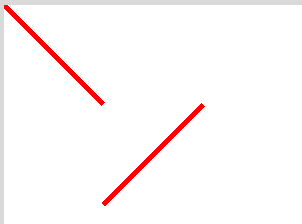
\includegraphics[scale=\myscale,scale=0.4]{ecran-tortue-1}
\end{center}	  
  
  \item Définis une \ci{tortue1} (rouge), une \ci{tortue2} (bleue).
  Définis une \ci{tortue3} (orange) qui à chaque déplacement de
  \ci{tortue1} et \ci{tortue2} se place au milieu de ces deux tortues.
  
  Sur le dessin ci-dessous : \ci{tortue1} se déplace en $(\frac32i,i)$ (pour 
  $i$ allant de $0$ à $400$) ; \ci{tortue2} se déplace successivement en $(i,5\sqrt{i})$.
  Pour chaque $i$, on récupère les positions de ces deux tortues et \ci{tortue3} se place au milieu.
 
  
\begin{center}
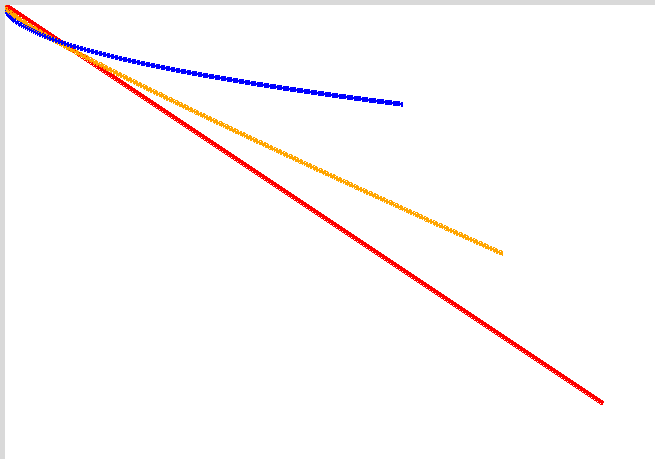
\includegraphics[scale=\myscale,scale=0.4]{ecran-tortue-2}
\end{center}	    

\end{enumerate}

Voici un exemple d'utilisation de notre tortue en utilisant le module \ci{tkinter} pour l'affichage (voir le dessin ci-dessus).
\begin{lstlisting}
from tkinter import *
root = Tk()      
canvas = Canvas(root, width=800, height=600, background="white")
canvas.pack(side=LEFT, padx=5, pady=5)

tortue = TortueBasique()

tortue.aller_a_xy(100,100)
tortue.relever_stylo()
tortue.aller_a_xy(200,100)
tortue.abaisser_stylo()
tortue.aller_a_xy(100,200)

root.mainloop()
\end{lstlisting}


\end{activite}

%%%%%%%%%%%%%%%%%%%%%%%%%%%%%%%%%%%%%%%%%%%%%%%%%%%%%%%%%%%%%%%%
%%%%%%%%%%%%%%%%%%%%%%%%%%%%%%%%%%%%%%%%%%%%%%%%%%%%%%%%%%%%%%%%


%%%%%%%%%%%%%%%%%%%%%%%%%%%%%%%%%%%%%%%%%%%%%%%%%%%%%%%%%%%%%%%%
%%%%%%%%%%%%%%%%%%%%%%%%%%%%%%%%%%%%%%%%%%%%%%%%%%%%%%%%%%%%%%%%

\begin{cours}[Programmation objet : héritage]

\index{programmation objet!heredité@hérédité}

La programmation objet possède un autre intérêt : à partir d'une classe d'objets on peut en définir d'autres, en récupérant certaines des fonctionnalités et en ajouter de nouvelles. C'est très utile par exemple pour reprendre et compléter du code écrit par d'autres. C'est la notion d'\defi{héritage}.

Voyons un exemple : on veut créer un jeu vidéo où il faut combattre des ennemis. Il y a différents types d'ennemis mais ils ont tous des caractéristiques communes : une position $(x,y)$ et des points de vie. 
Voici une classe \ci{Ennemi()} avec une méthode qui affiche les points de vie restant et une autre qui diminue les points de vie après avoir été attaqué.

\begin{lstlisting}
class Ennemi():
    def __init__(self,x,y,vie):
        self.x = x
        self.y = y
        self.vie = vie

    def affiche_vie(self):
        print("Vie =",self.vie)

    def perd_vie(self,n):
        self.vie = self.vie - n
\end{lstlisting}

Voici deux objets immobiles (des tours) définis par cette classe \ci{Ennemi()} 
et quelques actions.
\begin{lstlisting}
tour = Ennemi(1,2,100)
super_tour = Ennemi(5,3,200)
tour.affiche_vie()
tour.perd_vie(50)
tour.affiche_vie()
\end{lstlisting}

\medskip

Pour les ennemis passifs (qui peuvent être attaqués, mais ne peuvent pas attaquer)
la classe \ci{Ennemi()} est bien adaptée.
Par contre cette classe n'est pas assez évoluée pour des ennemis plus performants. Prenons l'exemple d'un zombie : en plus des caractéristiques déjà décrites, il est actif (il peut vous attaquer, se déplacer\ldots). Une solution est de programmer une classe \ci{Zombie()} depuis zéro, mais ce serait dommage car une partie du travail a été faite avec la classe \ci{Ennemi()}. Le plus simple est de récupérer les caractéristiques déjà existantes et d'en ajouter de nouvelles. C'est ce qu'on fait avec la classe \ci{Zombie()} qui hérite des propriétés de la classe \ci{Ennemi()} :

\begin{lstlisting}
class Zombie(Ennemi):
    def __init__(self,x,y,vie,force):
        Ennemi.__init__(self,x,y,vie)
        self.force = force

    def affiche_force(self):
        print("Force =",self.force)
\end{lstlisting}

Voici un exemple d'utilisation :

\begin{lstlisting}
mechant = Zombie(4,4,100,100)
mechant.affiche_force()
mechant.perd_vie(50)
mechant.affiche_vie()
\end{lstlisting}

Voici les explications : 
\begin{itemize}
  \item la classe \ci{Zombie()} est définie par l'entête \og{}\ci{class Zombie(Ennemi):}\fg{} et ainsi hérite des attributs et des méthodes de la classe \ci{Ennemi()}.
  
  \item Une instance de la classe \ci{Zombie()} possède les attributs \ci{x}, \ci{y} et \ci{vie} hérités de \ci{Ennemi()} mais possède en plus des points d'attaques stockés dans \ci{force}.
  
  \item La méthode \ci{__init__()} initialise un objet de la classe \ci{Zombie()}. Pour les caractéristiques déjà pré-existantes de la classe mère, on les initialise par \ci{Ennemi.__init__(self,x,y,vie)} et il ne reste plus qu'à initialiser \ci{force}.
  
  \item On définit une nouvelle méthode \ci{affiche_force()} qui concerne seulement les \ci{Zombie()}.
  
  \item On voit dans l'exemple d'utilisation comment définir un objet de la classe \ci{Zombie()} (avec ses quatre attributs). On peut bien sûr utiliser la méthode \ci{affiche_force()} spécifique à cette classe, mais aussi les méthodes \ci{affiche_vie()} et \ci{perd_vie()} héritées de la classe \ci{Ennemi()}.

\end{itemize}

\end{cours}

%%%%%%%%%%%%%%%%%%%%%%%%%%%%%%%%%%%%%%%%%%%%%%%%%%%%%%%%%%%%%%%%
% Activité 3
%%%%%%%%%%%%%%%%%%%%%%%%%%%%%%%%%%%%%%%%%%%%%%%%%%%%%%%%%%%%%%%%

\begin{activite}[Tortue tournante]

\index{tortue}

\objectifs{Objectifs : définir une tortue plus performante en se basant sur les propriétés de la tortue basique déjà construite.}

On veut améliorer la classe \ci{TortueBasique()} en une classe \ci{TortueTournante()} qui permet de diriger une tortue selon une direction.
La classe \ci{TortueTournante()} est donc héritée de la classe \ci{TortueBasique()} et un nouvel attribut \ci{direction} est créé.
Le début de la définition est donc :

\begin{lstlisting}
class TortueTournante(TortueBasique):
    def __init__(self):   
        TortueBasique.__init__(self)
        self.direction = 0
\end{lstlisting}        
       
L'attribut \ci{direction} correspond à l'angle en degrés vers lequel pointe la tortue. L'angle $0$ correspond à la droite, l'angle $90$ degrés correspond au Nord. % (ou au Sud selon la convention que tu as choisie).

\begin{enumerate}
  \item Complète la définition de la classe avec une méthode \ci{fixer_direction(self,direction)} qui met à jour la direction courante avec l'angle donné. 
  
  \emph{Encapsulation.} Cette fonction sert juste à éviter d'écrire \ci{tortue.direction = 90} ce qui est déconseillé en dehors de la définition de la classe. Il faut plutôt utiliser \ci{tortue.fixer_direction(90)}. Cette recommandation s'appelle l'\defi{encapsulation}.
	\index{programmation objet!encapsulation}
  
  \item Complète la définition de la classe avec une méthode \ci{tourner(self,angle)} qui change la direction courante en ajoutant l'angle donné. 
  
  \item Complète la définition de la classe avec une méthode \ci{avancer(self,longueur)}
  qui fait avancer la tortue de la longueur donnée selon sa direction courante.
  
  Voici les formules pour calculer les coordonnées $(x,y)$ du point d'arrivée en fonction du point de départ $(x_0,y_0)$ de la direction $\theta$ (en degrés) et de la longueur $\ell$ :
  $$x = x_0 + \ell \cos \left(\frac{2\pi}{360}\theta\right)  \qquad y = y_0 + \ell \sin\left(\frac{2\pi}{360}\theta\right) $$
 
 
\myfigure{1.3}{
\tikzinput{fig-tortue-1}
} 
    
  \item Complète la définition de la classe avec une méthode \ci{sorienter_vers(self,other)}
  qui oriente une tortue \ci{self} en direction de la tortue \ci{other}.
  
  
  \emph{Indications.} Si $(x_1,y_1)$ sont les coordonnées d'une première tortue, $(x_2,y_2)$ les coordonnées d'une seconde tortue alors l'angle formé entre l'horizontale et la droite joignant les deux tortues est donné (en degrés) par la formule :
  $$\theta = \frac{360}{2\pi} \operatorname{atan2}(y_2-y_1,x_2-x_1)$$
  où $\operatorname{atan2}(y,x)$ est une variante de la fonction arctangente disponible dans le module \ci{math}.
\myfigure{1.3}{
\tikzinput{fig-tortue-2}
} 
  
  Programme une poursuite de tortue : une tortue bleue descend pas à pas, à chaque étape la tortue rouge s'oriente vers la tortue bleue, puis avance. La courbe tracée par la tortue rouge s'appelle une \og{}courbe de poursuite\fg{}.
  
\begin{center}
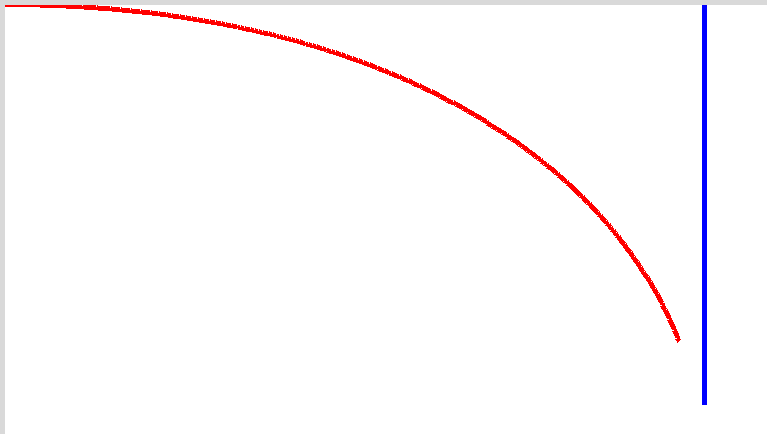
\includegraphics[scale=\myscale,scale=0.4]{ecran-tortue-3}
\end{center}	 
  
\end{enumerate} 

\end{activite}




\end{document}
